A knowledge discovery structure was carried out to standardise and arrange the knowledge discovery components of the study.
The Knowledge Discovery in Databases (KDD) process was utilised, in conjunction with the scikit-learn library \cite{scikit-learn} for data collection, preprocessing, dimensionality reduction, and algorithm implementation.
KDD is a five-stage\footnote{Some stages can be further split thus making a seven-stage process.} iterative process that outlines the data analysis life-cycle.


\subsection{Data Selection and Exploratory Analysis}\label{subsec:data-collection}
The source of the data set was obtained from Kaggle \cite{tsiaras2021ukroadsafety}, which is derived from the United Kingdom Department for Transport  \citetitle{roadtrafficdft} \cite{roadtrafficdft}.
The dataset contains accident data reporting to police where at least one person was injured and comes in two parts:
\begin{itemize}
    \item Accident data
    \item Vehicle data
\end{itemize}

We joined the two datasets on an \verb|Accident_Index| identifier.

\subsection{Data Pre-Processing}\label{subsec:data-pre-processing}

First of all we decided to remove records from 2004 as Vehicle information is missing from those records.
The dataset contains spatial coordinates in the form of Latitude and Longitude, and was subsequently used to inform the process of filling other missing data where appropriate.
There were a small number of missing Latitude/Longitude missing values to begin with - these were filled using the mode of the containing Local Area District.
In this way we maintained some element of location.
Once we had Latitude/Longitude complete we built a Nearest Neighbour structure using the entire dataset.
Missing values for the columns LSOA, Road Number, Speed Limit, Pedestrian Crossing and if in Scotland were imputed by querying the \verb|NearestNeighbour| structure for the nearest spatial neighbour(s) and setting the missing value based on that information.
We used \verb|sklearn.neighbours.BallTree| \cite{scikit-learn} to create the \verb|NearestNeighbour| structure based on latitude and longitude of all data (see Fig. \ref{fig:balltree}).


\begin{figure}[h]
    \centering
    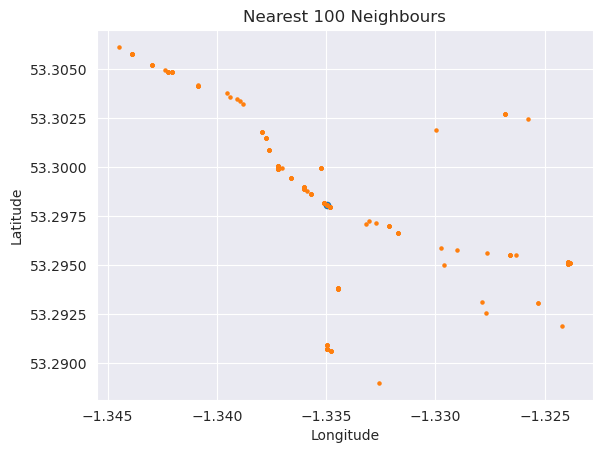
\includegraphics[width=0.5\textwidth]{images/Figure_BallTree}
    \caption{BallTree NearestNeighbour structure based on latitude and longitude}
    \label{fig:balltree}
\end{figure}

While this is slower than using mode or median, it does lead to far more accurate data.
Missing values for vehicle information was based on a loose hierarchy of Vehicle Type, Make, Model and Engine Capacity.
So for instance, when populating missing values for Model, we grouped by Make and used the mode of the group rather than the mode of the entire column.
To reduce the dataset and eliminate redundant variables, the following were removed:
\begin{itemize}
    \item Latitude/Longitude was used instead to fill missing data:
    \begin{itemize}
        \item Location Easting (OSGR)
        \item Location Northing (OSGR)
        \item Local Authority (District)
        \item Local Authority (Highway)
        \end{itemize}
    \item Dependent variables on top of the Accident Severity:
    \begin{itemize}
        \item Did Police Officer Attend Scene of Accident
        \item Number of Casualties
    \end{itemize}
    \item Irrelevant to our goal:
    \begin{itemize}
        \item Vehicle Reference
        \item LSOA of Accident Location
        \item Police Force
        \item In Scotland
        \item 1st Road Number
        \item 2nd Road Number
        \item Year
    \end{itemize}
    \item Related to other variables or made redundant after preprocessing:
    \begin{itemize}
        \item Time
        \item Latitude/Longitude
        \item Urban or Rural Area
    \end{itemize}
\end{itemize}

\subsection{Data Transformation}\label{subsec:data-transformation}

\begin{itemize}
    \item Numeric columns are standardised by scaling them between 0 and 1.
    \item Columns with only whole numbers converted from decimal to integer.
    \item \verb|Accident_Severity| is the dependent variable in our analysis, therefore Fatal and Serious were encoded as 1 and Slight to 0.
    \item Hour of Day $\rightarrow$  Early Morning, Late Morning, Early Afternoon, Late Afternoon, Evening, Night.
    \item Date $\rightarrow$ Day of Month, Day of Year
    \item Vehicle Type/Model and Engine Capacity $\rightarrow$ Commercial or Public Transport, Motorcycle, Regular Car, Sport Car, Large Engine Capacity Car, Small Engine Capacity Car, Other.
    \item And the remaining categorical columns were One-Hot encoded.
\end{itemize}

The data transformation process resulted in a total of 219 features for us to then analyse further.

\subsection{Data Mining}\label{subsec:data-mining}

We conducted a Chi-square test on each feature to assess which ones reject or fail to reject the null hypothesis ($H0$).
We conduced a Ch-square test to identify which features (e.g., road conditions, weather, vehicle type, etc.) have a significant relationship with accident severity.
The test uses a significance level of $\alpha=0.05$.

If the p-value is less than or equal to 0.05, it is concluded that there is a significant relationship between the feature and accident severity.
The critical value is another approach to deciding about the null hypothesis.
If the Chi-square statistic is greater than the critical value, the null hypothesis is rejected, indicating that the feature has a significant impact on accident severity.

Each feature is analysed, and its Chi-square statistic, p-value, degrees of freedom, and critical value are calculated.
Based on these values, the features are classified into two groups: those with a significant relationship to accident severity and those without a significant relationship.
This classification is done using both the critical value and the p-value methods, but either one works since both should match up.

We also used the Recursive Feature Elimination (RFE) technique to identify which features are more relevant for predicting the severity of an accident.
Computing the ANOVA F-value was considered initially, but computing Chi-square statistics was preferred due to the nature of the binary input.
The process was to split the data into training and testing and use the best $k$ features for predicting our target class.
The value $k$ started by including all of our features and iteratively reduce $k$ by one for each prediction.
The Bernoulli Naive Bayes classifier was used since it is fast and suitable for one-hot encoded data and the recall value was recorded.
The recall value was preferred over the F1, accuracy and precision since we wanted to ensure that false negatives would be minimised.
Recall measures the proportion of actual positive outcomes (severe/fatal) that are correctly identified by our classifier and helps us capture a larger percentage of the true positive outcomes.